\documentclass{article}

\usepackage{microtype}
\usepackage{graphicx}
\usepackage{booktabs}
\usepackage{hyperref}
\usepackage[accepted]{icml2018}
\usepackage{amsmath}

\begin{document}

\twocolumn[
\icmltitle{Reinforcement Learning on Hanabi}

\begin{icmlauthorlist}
\icmlauthor{Saanvi Chawla}{Stanford University}
\icmlauthor{Tanmay Garg}{Stanford University}
\icmlauthor{Arunima Srivastav}{Stanford University}
\end{icmlauthorlist}

\icmlaffiliation{Stanford University}{Stanford University, CA, USA}
\icmlcorrespondingauthor{Tanmay Garg}{tanmayg@stanford.edu}
\icmlcorrespondingauthor{Saanvi Chawla}{saanvic@stanford.edu}
\icmlcorrespondingauthor{Arunima Srivastava}{aru04@stanford.edu}

\vskip 0.3in
]

\printAffiliationsAndNotice{}

\section{Introduction}

Hanabi has become a canonical benchmark for cooperative multi-agent reinforcement learning (MARL) under partial observability \cite{bard2019hanabi}: players cannot observe their own hands and must coordinate through sparse, structured hints that serve simultaneously as game actions and communication signals. Agents trained via self-play can achieve strong performance, but the resulting conventions are typically opaque, brittle under partner mismatch, and difficult to transfer to human partners. \\

Sudhakar et al.~\cite{sudhakar2025generalist} show that self-play agents develop sophisticated signaling behaviors that score well yet remain poorly understood — the internal structure of the learned protocols is unclear, and these conventions do not transfer reliably to humans or novel partners. Strong in-distribution performance, in other words, does not imply interpretable or generalizable coordination. \\

This motivates a natural pair of questions: what structure do learned conventions actually exhibit, and can we regularize toward simpler, more human-compatible signaling without sacrificing performance? We build on the training and evaluation pipeline of Sudhakar et al. For the milestone, we focus on interpretability. By analyzing which features the agent attends to and how that attention is distributed across game phases and action types, we aim to understand where the complexity in the learned policy  actually comes from. Beyond the milestone, we plan to use those findings directly to design a 
complexity-aware regularization term in the RL objective. Rather than penalizing complexity arbitrarily, the goal is for the interpretability analysis to ground what we penalize and why.

\section{Approach}

We are continuing our work in the text-based environment used by \cite{sudhakar2025generalist}. There are 3 types of actions: play a card, discard a card, and give a clue. We encode the action with a keyword corresponding to the action-type, followed by the type’s parameter (e.g. reveal blue 2). We begin our work on interpretability by using the 2 player model checkpoint provided by \cite{sudhakar2025generalist}.\\

We define the 7 important parts of our Hanabi game state that an agent would need to reason about before making its next action. First, life tokens, which indicate the number of mistakes remaining in the game. Second, hint tokens, which indicate number of hints remaining. Third, fireworks, which contain the progress so far on each color stack. Fourth, the agent's own hand, the information agent has on its hand through the opponent's hints. Fifth, the opponent's hand, the complete information an agent has on opponent's hand. Sixth, discards, the cards which have been discarded so far. Lastly, the previous action, which is the most recent move made in the game.

Using these, we define 4 statistics for a Hanabi game and use them as proxies for the complexity of the strategy used by our pre-trained Hanabi agent:

\begin{itemize}
    \item $p_i = \frac{|IG_i|}{\sum_j IG_j}$ where $IG_k$ is the integrated gradient for section $k$ (there are 7 sections from above). $p_i$ represents the fraction of total decision signal coming from section $i$. We then define the entropy of the agent $H(p) = -\sum_i p_i \log(p_i)$ where a higher entropy indicates a more complex policy being followed by the agent.
    \item Effective feature count: $2^H$
    \item Gini coefficient: this is used to answer the question about how concentrated the agent's decision is among the 7 sections. We define $C_i = \sum_{j=0}^i p_i$, i.e., the sum of the i smallest scores. Then, we get the gini coefficient = $1 - \frac{2}{n} \sum_i C_i$.
    \item Top 2 dominance captures the fraction of total attribution captured by the top 2 most-attended sections. This fraction will be higher for simpler policies where the top 2 features explain most of the reasoning in the decision. Thus, the formula for the top 2 dominance = $\frac{\texttt{largest}(IG) + \texttt{second-largest}(IG)}{\sum_j IG_j}$.
\end{itemize}

% Describe the environment or dataset, the algorithms being implemented, and the overall technical setup. Include mathematical formulation or architecture details if relevant.

% Explain what has already been implemented, what is working, and any preliminary observations or results.

% Here's the revised Current Progress section focused on your Phase 3 complexity diagnostics results:

\section{Current Progress}

\subsection{Architecture Primer}

There are 21 actions in the 2-player setting: discard cards 0--4 (D1--D5), play cards 0--4 (P1--P5), hint color to partner (CR, CY, CG, CW, CB), hint rank to partner (R1--R5), and noop.

\subsection{Complexity Diagnostics}

We evaluated our statistics across four game phases: early game, mid game, late game, and crisis (when we have only 1 life token, 0 hint tokens), and five probe actions per phase: greedy, D1, P1, CR, R1.

\subsection{Results}

\subsubsection{Overall Feature Reliance}

The agent's attribution is distributed across all seven game-state sections: discards (30.7\%), opponent's hand (16.6\%), life tokens (15.6\%), fireworks (15.2\%), own hand (12.3\%), hint tokens (6.0\%), and last action (3.6\%). Despite a clear rank ordering, five of seven sections individually exceed 10\%, and even the top section captures less than a third of total attribution. The overall mean entropy of 2.533 bits represents 90.2\% of the theoretical maximum, with every action--phase cell exceeding 2.3 bits, confirming uniformly distributed reliance across features.

\begin{figure}[h]
    \centering
    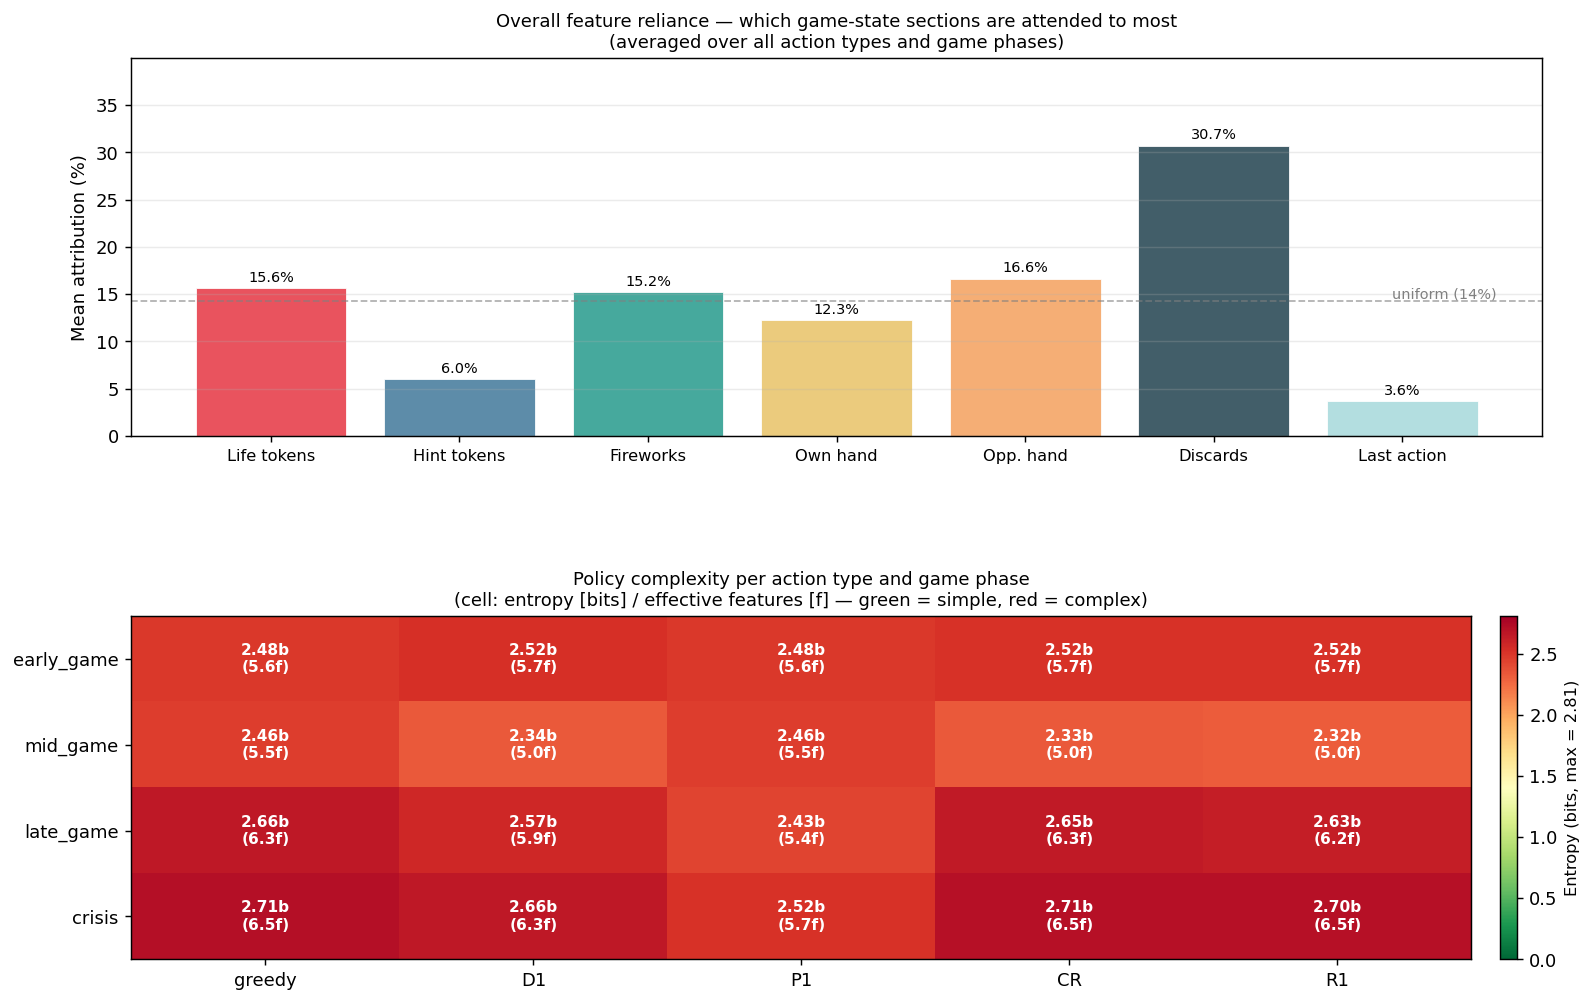
\includegraphics[width=\columnwidth]{complexity_results/diag5_summary.png}
    \caption{Top: mean attribution percentage per game-state section, averaged over all actions and phases. The dashed line marks the uniform baseline (14\%). Bottom: entropy (bits) and effective feature count per action type and game phase. All cells are deep red, indicating uniformly high complexity.}
    \label{fig:summary}
\end{figure}

\subsubsection{Attribution Heatmaps Across Game Phases}

Attribution heatmaps across the four game phases reveal near-uniform rows for most conditions, indicating high-complexity multi-feature decisions throughout. Mid-game shows the most structure, with discards capturing 31--46\% of attribution depending on the action, reflecting the discard pile's informativeness at that stage. Play actions (P1) consistently show the most concentrated attribution, while hint actions remain the most uniform. Late game and crisis phases flatten again as game constraints tighten.

\begin{figure}[h]
    \centering
    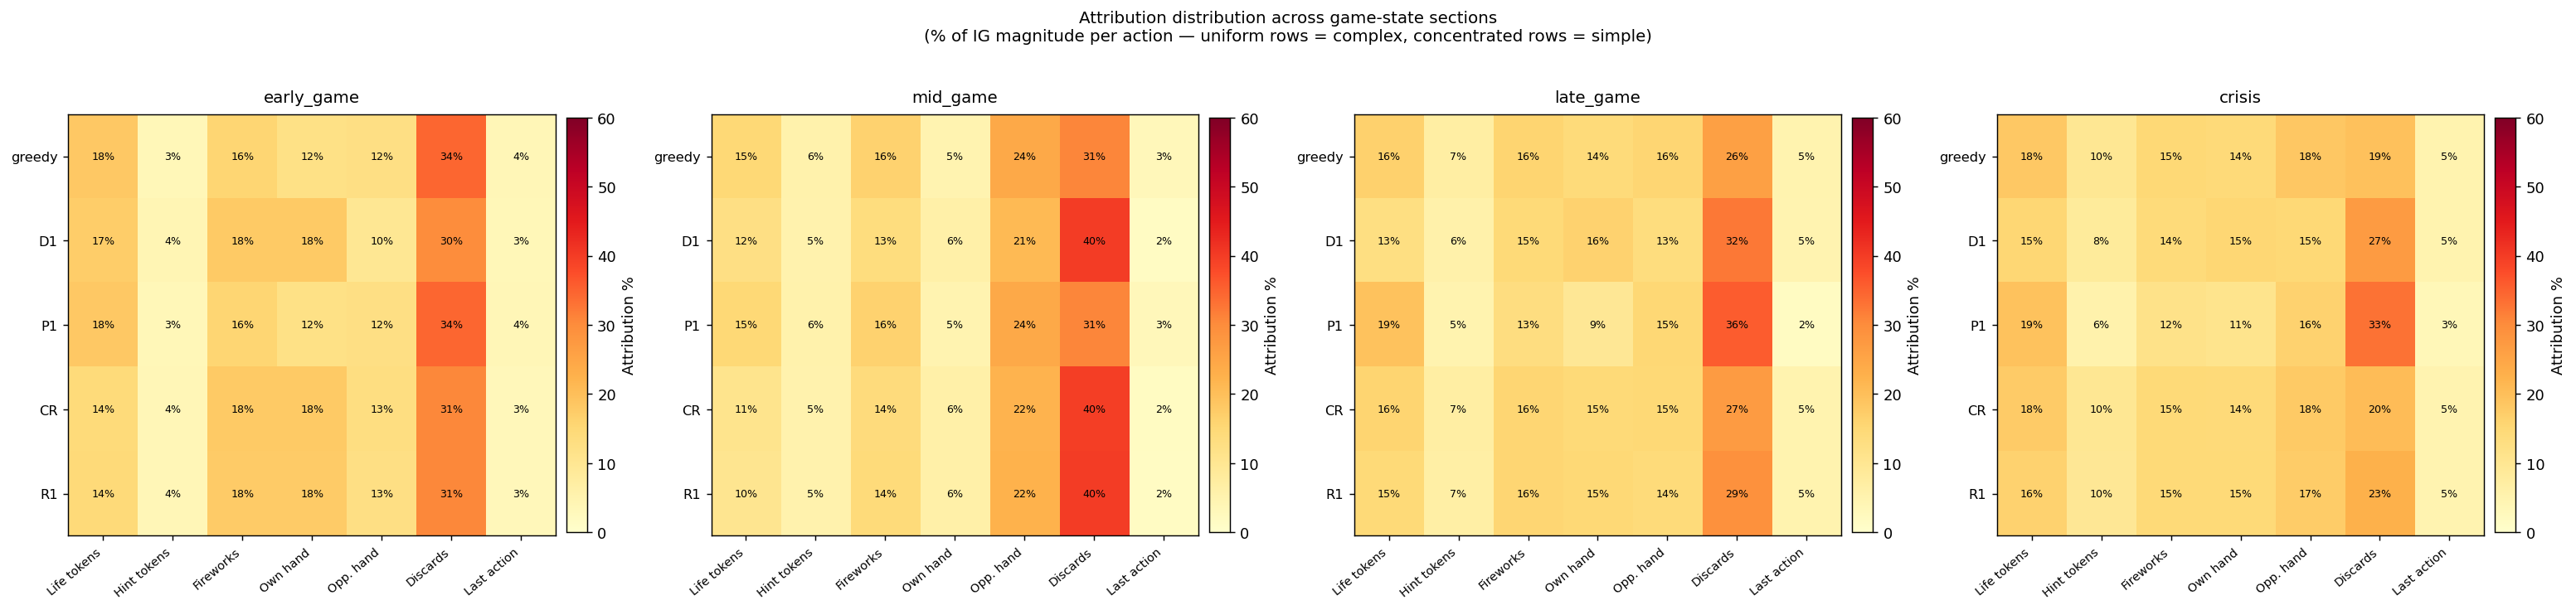
\includegraphics[width=\columnwidth]{complexity_results/diag1_heatmap.png}
    \caption{Attribution distribution for each action type. Uniform rows indicate complex, multi-factor decisions, concentrated rows indicate simpler decisions.}
    \label{fig:heatmap}
\end{figure}

\subsubsection{Entropy and Effective Feature Count}

All action--phase entropy values exceed $\log_2(5) = 2.32$ bits, meaning every action effectively consults at least 5 features. The human-learnable target of $H \leq 1.58$ bits ($\leq$3 features) lies 0.8--1.2 bits below all measured values. Entropy follows a non-monotonic pattern across phases: mid-game is lowest (2.378 bits, $N_{\text{eff}} = 5.14$) due to focused discard and opponent-hand signals, while crisis is highest (2.659 bits, $N_{\text{eff}} = 6.33$) as flat Q-values spread attribution uniformly.

\begin{figure}[h]
    \centering
    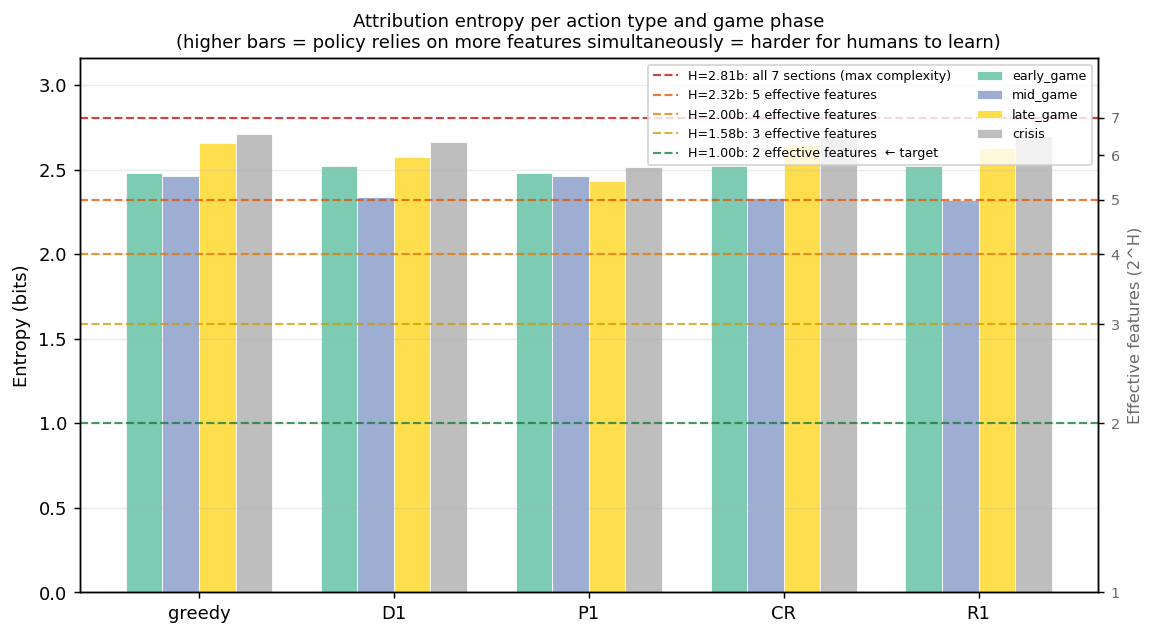
\includegraphics[width=\columnwidth]{complexity_results/diag2_entropy.png}
    \caption{Attribution entropy (bits) per action type and game phase. Reference lines show the entropy corresponding to 2, 3, 4, 5, and 7 effective features. All bars exceed the 5-feature line; the human-learnable target of $\leq 3$ features ($H \leq 1.58$ bits) is far below.}
    \label{fig:entropy}
\end{figure}

\subsubsection{Concentration Curves}

Cumulative attribution curves show that no action--phase pair reaches the target of top-2 sections capturing $\geq$80\% of total attribution. The top-1 section captures only 25--35\%, and the top-2 together only 38--62\%. P1 in mid-game approaches the target fastest (reaching 80\% by top-3 sections), while the noop action in crisis is flattest, requiring top-5 or top-6 sections. No simple 2--3 feature rule can approximate the agent's decisions.

\begin{figure}[h]
    \centering
    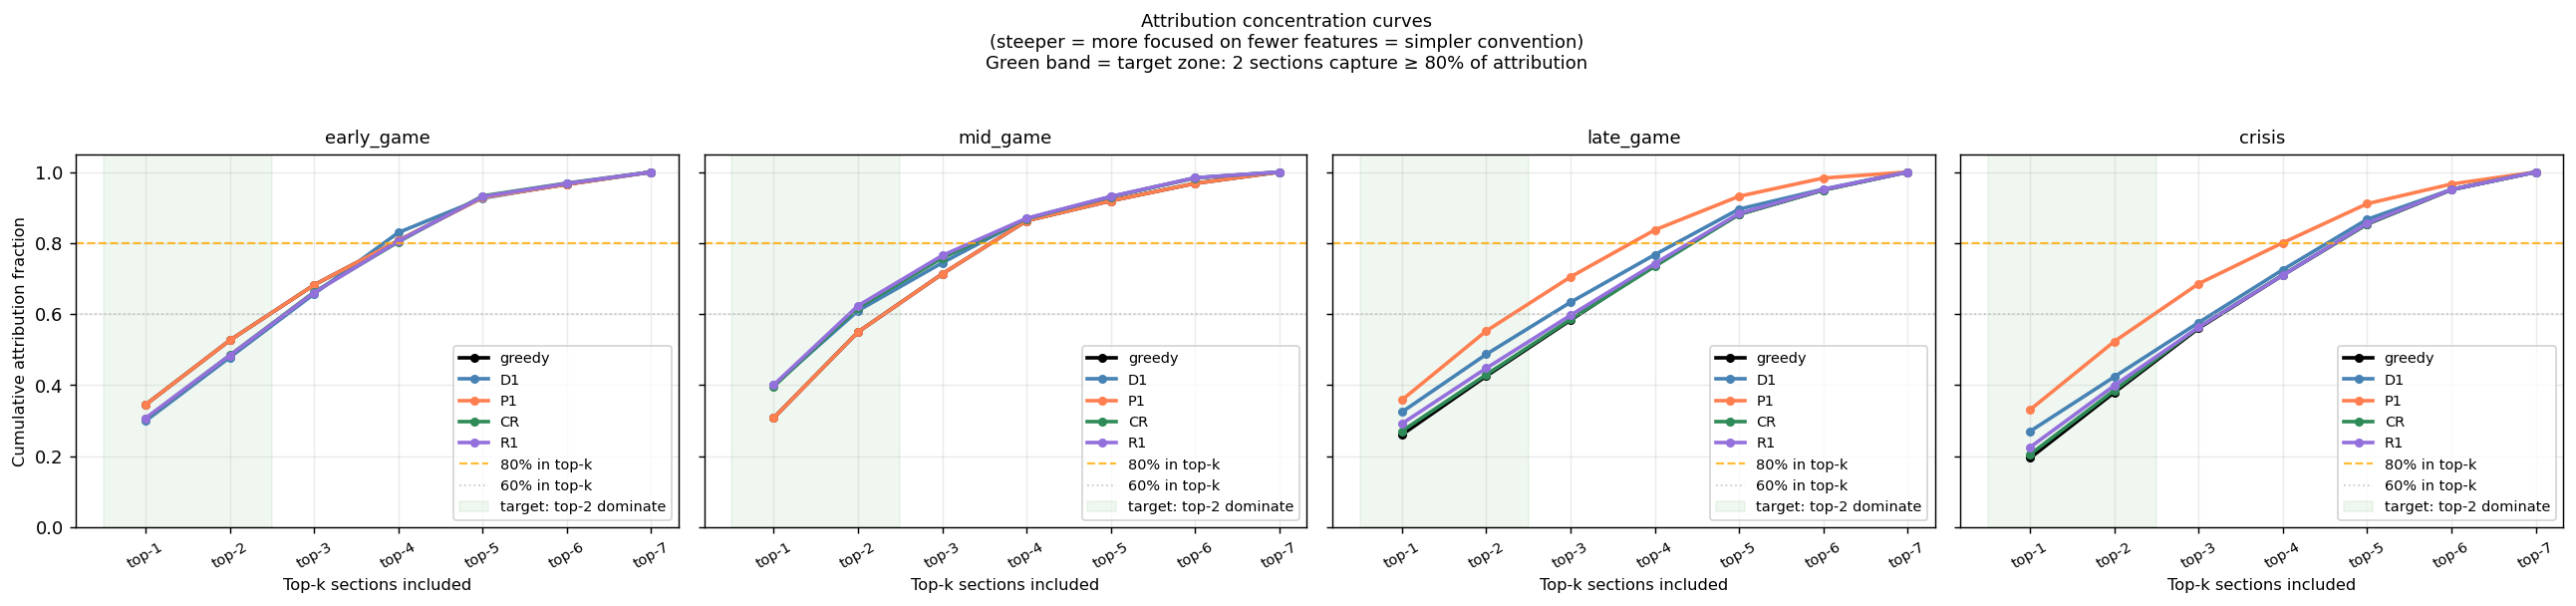
\includegraphics[width=\columnwidth]{complexity_results/diag4_concentration.png}
    \caption{Cumulative attribution curves showing how rapidly total attribution concentrates in the top-ranked sections. The green band marks the target zone (top-2 sections $\geq$ 80\%). No action--phase pair enters the target zone, with the gap ranging from 18 to 42 percentage points.}
    \label{fig:concentration}
\end{figure}

\subsubsection{Concentration Metrics: Gini Coefficient and Top-2 Dominance}

Both metrics are consistent, the agent's decisions are far from concentrated. Gini coefficients range from 0.185 (noop in crisis) to 0.450 (R1 in mid-game), well below the values expected of a focused policy. Top-2 dominance peaks at 62.4\% (R1, mid-game) and falls as low as 37.9\% (noop, crisis), leaving a gap of at least 18 percentage points from the 80\% target that would indicate a policy explainable by two features. Mid-game produces the highest concentration across all metrics, consistent with discards and opponent's hand jointly dominating that phase. Crisis produces the lowest concentration: with a flat Q-value landscape and no clearly dominant action, attribution spreads nearly uniformly and the Gini coefficient approaches zero. P1 (play) is consistently the most concentrated action across all phases, while noop and hint actions (CR, R1) are the most diffuse---no simple 2-feature rule approximates the agent's reasoning in any condition.

\section{Remaining Work}

Having established that the trained agent exhibits a high-complexity policy, consulting nearly six out of seven input features simultaneously regardless of 
game phase or action type, our remaining work focuses on two goals: completing the interpretability characterization and using those findings to guide 
complexity-penalized retraining. \\

On the interpretability side, we plan to extend the current integrated gradients analysis to cross-play settings, where agents trained via self-play are paired with partners using different conventions. We will run IG attribution on games between two independently trained self-play agents and compare the resulting entropy and top-2 dominance distributions against the self-play baseline reported above. Our hypothesis is that the diffuse attribution structure we observe reflects conventions that are over-fitted to a specific partner's signaling patterns. Thus, when paired with a mismatched partner, the agent will show increased entropy and degraded top-2 dominance as it fails to find a reliable information source to anchor its decisions. If this holds, simpler conventions would not only be easier for humans to follow, but more robust to partner mismatch, giving us a concrete functional motivation for the regularization work that follows.

On the regularization side, we plan to introduce a complexity penalty into the RL objective that discourages the agent from spreading its attention across too many features at once. Our diagnostics suggest a natural target of keeping attribution entropy below $\log_2(3) \approx 1.58$ bits, which corresponds to relying on at most three features effectively. We treat this as a rough threshold for conventions a human could plausibly learn. The practical challenge is that integrated gradients are too expensive to compute at every training step -- running 20 forward passes per decision would make training prohibitively slow. Instead, we will explore cheaper proxies, most likely a learned attention layer over the seven input sections whose entropy can be penalized directly in a single forward pass. We will train agents under a range of penalty strengths $\lambda$ and trace out the resulting score-vs-entropy tradeoff, using cross-play performance as the key test of whether simpler conventions actually generalize better. The goal is to identify the point on that curve where the agent is still playing well but relying on a focused, legible set of features.

% \bibliographystyle{icml2018}
\bibliographystyle{abbrvnat}
\bibliography{references}

\section{Appendix}

\begin{table}[h]
\centering
\caption{Gini coefficient and Top-2 dominance (\%) by action type and game phase. Higher Gini and Top-2 values indicate more focused, interpretable decisions.}
\label{tab:concentration}
\resizebox{\columnwidth}{!}{%
\begin{tabular}{llccccc}
\toprule
\textbf{Phase} & \textbf{Metric} & \textbf{greedy} & \textbf{D1} & \textbf{P1} & \textbf{CR} & \textbf{R1} \\
\midrule
Early  & Gini          & 0.358 & 0.331 & 0.358 & 0.330 & 0.330 \\
       & Top-2 (\%)    & 52.6  & 47.8  & 52.6  & 48.4  & 48.4  \\
\midrule
Mid    & Gini          & 0.377 & 0.439 & 0.377 & 0.444 & 0.450 \\
       & Top-2 (\%)    & 55.0  & 61.0  & 55.0  & 61.8  & 62.4  \\
\midrule
Late   & Gini          & 0.239 & 0.302 & 0.390 & 0.243 & 0.260 \\
       & Top-2 (\%)    & 42.5  & 48.7  & 55.2  & 42.9  & 44.7  \\
\midrule
Crisis & Gini          & 0.185 & 0.232 & 0.348 & 0.191 & 0.201 \\
       & Top-2 (\%)    & 37.9  & 42.3  & 52.3  & 38.5  & 39.9  \\
\bottomrule
\end{tabular}}
\end{table}


\begin{figure}[h]
    \centering
    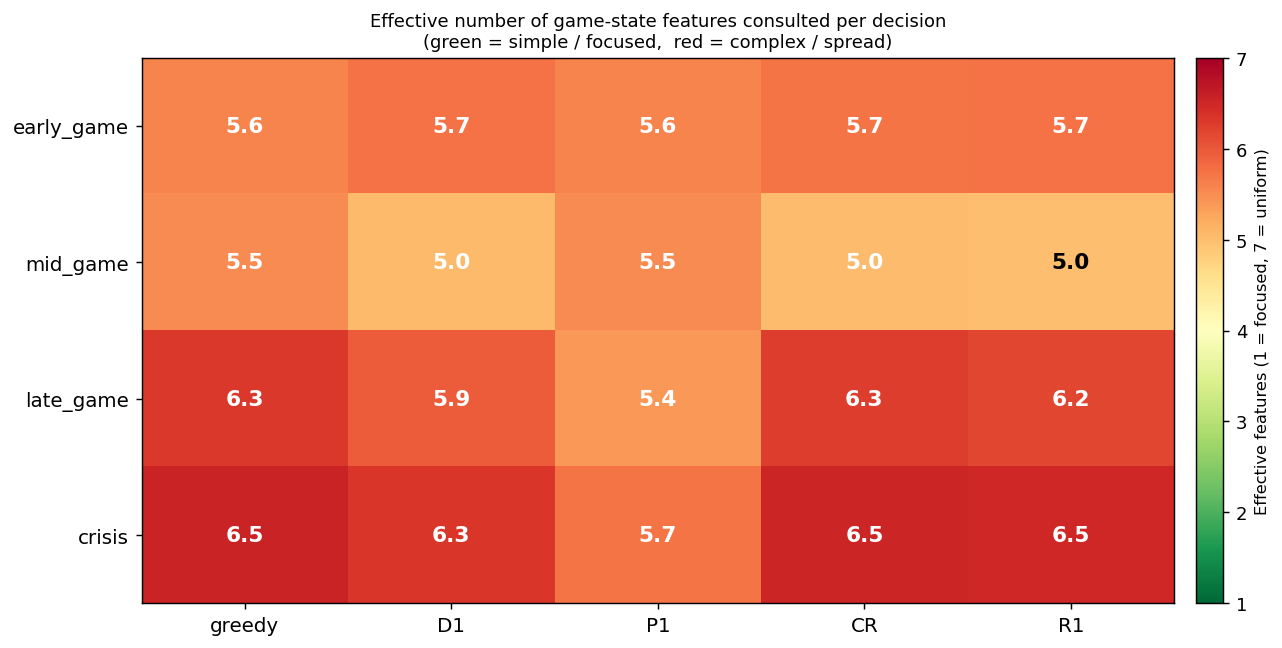
\includegraphics[width=\columnwidth]{complexity_results/diag3_effective_n.png}
    \caption{Effective feature count ($2^H$) per action type and game phase. Green indicates focused attention (few features); red indicates diffuse attention (many features). The grid is uniformly red-orange, ranging from 5.0 (mid-game hint actions) to 6.5 (crisis).}
    \label{fig:effective_n}
\end{figure}

\end{document}